\documentclass[11pt,a4paper]{article}
\usepackage[margin=2.2cm]{geometry}
\usepackage{booktabs}
\usepackage{graphicx}
\usepackage{xcolor}
\usepackage[colorlinks=true,linkcolor=clinteal,urlcolor=clinteal]{hyperref}
\usepackage{longtable}
\usepackage{enumitem}
\usepackage{fancyhdr}
\usepackage{titlesec}
\usepackage{caption}
\usepackage{subcaption}
\usepackage{float}
\usepackage{parskip}

\definecolor{clinred}{RGB}{213,94,0}
\definecolor{clinamber}{RGB}{230,159,0}
\definecolor{clingreen}{RGB}{0,158,115}
\definecolor{clinteal}{RGB}{0,119,182}

\captionsetup{font=small, labelfont=bf, textfont=it}

\pagestyle{fancy}
\fancyhf{}
\rhead{\small Neuropsychological Report}
\lhead{\small subj\_048}
\rfoot{\thepage}

\titleformat{\section}{\Large\bfseries\color{clinteal}}{\thesection}{1em}{}
\titleformat{\subsection}{\large\bfseries\color{clinteal!70!black}}{\thesubsection}{1em}{}
\titleformat{\paragraph}[runin]{\normalsize\bfseries\color{clinteal!60!black}}{}{0em}{}[.]

\begin{document}

\begin{center}
{\LARGE\bfseries Neuropsychological Assessment Report}\\[0.5em]
{\large Subject: subj\_048}\\[0.3em]
{\normalsize Date of Report: \today}
\end{center}

\vspace{0.5em}
\noindent\rule{\textwidth}{0.4pt}

% ================================================================
\section{Demographics and Clinical Context}
% ================================================================

\begin{tabular}{ll}
\textbf{Age:} & 31 years \\
\textbf{Gender:} & F \\
\textbf{Group:} & IBS \\
\textbf{IBS Subtype:} & M \\
\textbf{IBS Severity (SSS):} & 305 \\
\end{tabular}

\medskip\noindent Patient belongs to the IBS group (n=65 of 105 total). IBS subtype: M (n=32 in cohort). Age 31 (cohort M=37.0, SD=11.8). 

% ================================================================
\section{Domain Findings}
% ================================================================

\subsection{Sleep --- Bergen Insomnia Scale (BIS)}
BIS total = 32.0 (Severe). Cohort percentile: 98th. z = +2.13. This indicates clinically significant insomnia symptoms that likely impact daytime functioning and cognitive performance.

\noindent\begin{tabular}{llll}
\textbf{BIS Total:} & 32.0 &
\textbf{Classification:} & \textbf{Severe} \\
\textbf{Cohort percentile:} & 97.9th &
\textbf{Cohort z-score:} & $2.13$ \\
\end{tabular}

\subsection{Sustained Attention --- Continuous Performance Test (CPT)}
CPT Detectability (d') T=46.0 (47th percentile in cohort, z=-0.15). All CPT metrics within normal limits. Sustained attention and response control appear intact.

\begin{table}[H]
\centering\small
\begin{tabular}{lccc}
\toprule
\textbf{CPT Metric} & \textbf{T-score} & \textbf{Cohort \%ile} & \textbf{Status} \\
\midrule
    Signal detection sensitivity (d') & T=46.0 & 47.1 & \textcolor{clingreen}{Normal} \\
    Missed targets (inattention) & T=45.0 & 44.1 & \textcolor{clingreen}{Normal} \\
    False alarms (impulsivity) & T=52.0 & 64.2 & \textcolor{clingreen}{Normal} \\
    Mean reaction time & T=52.0 & 73.5 & \textcolor{clingreen}{Normal} \\
    Reaction time variability & T=50.0 & 80.4 & \textcolor{clingreen}{Normal} \\
    Anticipatory responses & T=48.0 & 73.5 & \textcolor{clingreen}{Normal} \\
    Response speed consistency & T=51.0 & 85.6 & \textcolor{clingreen}{Normal} \\
\bottomrule
\end{tabular}
\caption{CPT-3 performance metrics. T-scores are normed (M=50, SD=10). Higher T-scores indicate less favorable performance across the displayed CPT metrics. Scores $\geq$60 are mildly elevated; $\geq$65 are clinically significant.}
\end{table}

\subsection{Fatigue --- Chalder Fatigue Scale}
Chalder Fatigue bimodal total = 11.0 (11/11 items endorsed). Classification: Significant fatigue. Cohort percentile: 97th. Clinically significant fatigue present. This may impact attention, processing speed, and overall cognitive efficiency.

\noindent\begin{tabular}{llll}
\textbf{Bimodal total:} & 11.0/11 &
\textbf{Classification:} & \textbf{Significant fatigue} \\
\textbf{Cohort percentile:} & 97.0th &
\textbf{Caseness threshold:} & $\geq$4 \\
\end{tabular}

\subsection{Emotional Distress --- Hospital Anxiety and Depression Scale (HADS)}
HADS Anxiety = 12.0 (Clinical, 85th \%ile). HADS Depression = 6.0 (Normal, 77th \%ile). Clinically significant emotional distress present. This is likely to affect cognitive test performance, particularly attention and executive function.

\noindent\begin{tabular}{lllll}
 & \textbf{Score} & \textbf{Classification} & \textbf{Cohort \%ile} & \textbf{z-score} \\
\textbf{HADS-A:} & 12.0 & Clinical & 85.5th & $1.27$ \\
\textbf{HADS-D:} & 6.0 & Normal & 76.9th & $0.75$ \\
\end{tabular}

\smallskip\noindent\small Cutoffs: 0--7 Normal; 8--10 Borderline; 11--21 Clinical caseness.

\subsection{Neurocognition --- RBANS}
RBANS Sum Raw = 213.0 (14.7th cohort percentile). Interpretation is based on the cleaned dataset's raw subtests and cohort-relative summaries rather than the older RBANS index-score fields. Relative weaknesses are most evident in Immediate Memory, Language, Delayed Memory, Recognition. 

\begin{table}[H]
\centering\small
\begin{tabular}{lccc}
\toprule
\textbf{Index} & \textbf{Score} & \textbf{Cohort \%ile} & \textbf{Classification} \\
\midrule
    Immediate Memory & -0.55 & 22.1 & Relative weakness \\
    Visuospatial & 0.06 & 45.6 & Mid cohort position \\
    Language & -1.32 & 5.9 & Marked relative weakness \\
    Attention & -0.09 & 46.1 & Mid cohort position \\
    Delayed Memory & -0.84 & 17.2 & Relative weakness \\
    Recognition & -0.41 & 24.0 & Relative weakness \\
    Total Scale & 213.0 & 14.7 & Relative weakness \\
\bottomrule
\end{tabular}
\caption{RBANS summary values in the standalone March 16 pipeline. Domain scores reflect cohort-standardized raw-subtest composites, and ``Total Scale'' reflects RBANS Sum Raw. Classifications describe relative position within the observed cohort rather than external age-corrected norms.}
\end{table}

% ================================================================
\section{Clinical Flags}
% ================================================================
\textbf{Sleep (BIS):}
\begin{itemize}[leftmargin=2em, topsep=0pt]
  \item Clinically elevated insomnia
  \item Above clinical threshold ($\geq$19)
  \item Multiple items $\geq$3 days/week: Q2, Q3, Q4, Q5, Q6
\end{itemize}
\textbf{Fatigue (Chalder):}
\begin{itemize}[leftmargin=2em, topsep=0pt]
  \item Chalder caseness (bimodal total=11 $\geq$ 4)
\end{itemize}
\textbf{Emotional Distress (HADS):}
\begin{itemize}[leftmargin=2em, topsep=0pt]
  \item HADS-A clinical (12)
\end{itemize}
\textbf{Neurocognition (RBANS):}
\begin{itemize}[leftmargin=2em, topsep=0pt]
  \item Language: marked relative weakness within cohort
  \item RBANS Sum Raw falls in the lowest cohort range
\end{itemize}


% ================================================================
\section{Cross-Domain Pattern Analysis}
% ================================================================
Insomnia-fatigue co-occurrence: Elevated BIS and Chalder scores together suggest that poor sleep is driving daytime fatigue. Although CPT performance is currently preserved, this combination places the patient at risk for developing attentional difficulties if sleep disturbance persists (Fortier-Brochu et al., 2012). Mood-cognition interaction: Emotional distress (HADS) co-occurs with cognitive difficulties. Anxiety consumes working memory resources through worry-related rumination, while depression slows processing speed and impairs encoding (Castaneda et al., 2008). Both mechanisms can degrade performance on RBANS and CPT independently of any organic pathology. Mood-sleep bidirectional relationship: Both insomnia and emotional distress are elevated, consistent with their well-documented bidirectional association (Baglioni et al., 2011). Insomnia is both a symptom and a maintaining factor for anxiety and depression; treating sleep may yield secondary mood benefits and vice versa. Gut-brain axis involvement: As an IBS patient with elevated scores in sleep, fatigue, mood, this profile is consistent with gut-brain axis mediated effects. IBS-associated visceral hypersensitivity activates the hypothalamic-pituitary-adrenal (HPA) axis and alters serotonergic signaling, which can drive insomnia, fatigue, and affective dysregulation (Mayer et al., 2015). An integrated treatment approach addressing both gastrointestinal and neuropsychological symptoms is warranted.

% ================================================================
\section{Clinical Reasoning Chain}
% ================================================================

The following reasoning chain traces the step-by-step clinical logic used to integrate findings across domains, identify mechanistic links, and arrive at the recommendations below.

\paragraph{Step 1: Demographic and clinical context}
F, age 31, IBS group, IBS subtype M. IBS-SSS=305.

\paragraph{Step 2: Sleep (BIS)}
Total score 32.0, classified as Severe (cohort 97.9th percentile).

\paragraph{Step 3: Fatigue (Chalder)}
Bimodal total 11.0, Significant fatigue (cohort 97.0th percentile).

\paragraph{Step 4: Emotional distress (HADS)}
Anxiety 12.0 (Clinical), Depression 6.0 (Normal).

\paragraph{Step 5: Sustained attention (CPT)}
Detectability T=46.0, Omissions T=45.0, Commissions T=52.0, HRT T=52.0.

\paragraph{Step 6: Neurocognition (RBANS)}
Sum Raw 213.0 at the 14.7th cohort percentile. The interpretation uses raw subtests plus cohort-standardized summary composites. Relative weaknesses are present in Immediate Memory, Language, Delayed Memory, Recognition, Total Scale.

\paragraph{Step 7: Cross-domain integration}
Flags span sleep, fatigue, mood, cognition, supporting an interacting symptom pattern.

\paragraph{Step 8: Prognostic formulation}
Mood and cognitive inefficiency co-occur, so emotional stabilization may improve concentration and reduce apparent cognitive burden.



% ================================================================
\section{Recommendations Based on Pre-Screening Results}
% ================================================================

Each recommendation below is explicitly linked to the pre-screening domain finding(s) that justify it. Domain labels in \textbf{bold} indicate the driving finding. Recommendations follow a two-stage structure: (1)~determine whether further examination is necessary, then (2)~outline treatment planning and interventions.

\subsection{Further Examinations or Referrals Recommended}
\begin{itemize}[leftmargin=*]
  \item \textbf{COGNITION:} Follow up the cohort-relative RBANS weaknesses in Immediate Memory, Language, Delayed Memory, Recognition, Total Scale if the patient reports matching day-to-day difficulties.
  \item \textbf{COGNITION:} If cognitive complaints persist despite treating sleep, fatigue, and mood contributors, consider expanded neuropsychological assessment.
  \item \textbf{IBS:} High symptom burden supports close gastroenterology follow-up alongside symptom-targeted psychological care.
\end{itemize}

\subsection{Suggested Therapeutic Interventions}
\begin{itemize}[leftmargin=*]
  \item \textbf{SLEEP:} Prioritize CBT-I and structured sleep-hygiene measures, as insomnia is a likely upstream driver of daytime fatigue and reduced cognitive efficiency.
  \item \textbf{FATIGUE:} Use paced activity scheduling and screen for reversible medical contributors such as anemia, thyroid disease, and vitamin deficiency.
  \item \textbf{FATIGUE-SLEEP LINK:} Reassess fatigue after sleep-focused treatment before escalating to more extensive fatigue workup.
  \item \textbf{ANXIETY:} Consider CBT-based anxiety treatment; anxious arousal can worsen sleep and concentration.
  \item \textbf{IBS INTEGRATION:} Coordinate neuropsychological follow-up with gastrointestinal care, since gut-brain symptoms may reinforce sleep, fatigue, and mood burden.
\end{itemize}

% ================================================================
\newpage
\section{Visualizations}
% ================================================================

Three pairs of complementary figures are provided, each tailored to a specific audience.
All scores are shown in the context of the full cohort (N=105), split by IBS status (n=65) vs. healthy controls (n=40).

% --- A. CLINICAL AUDIENCE ---
\subsection{For Clinical Peers}

\begin{figure}[H]
\centering
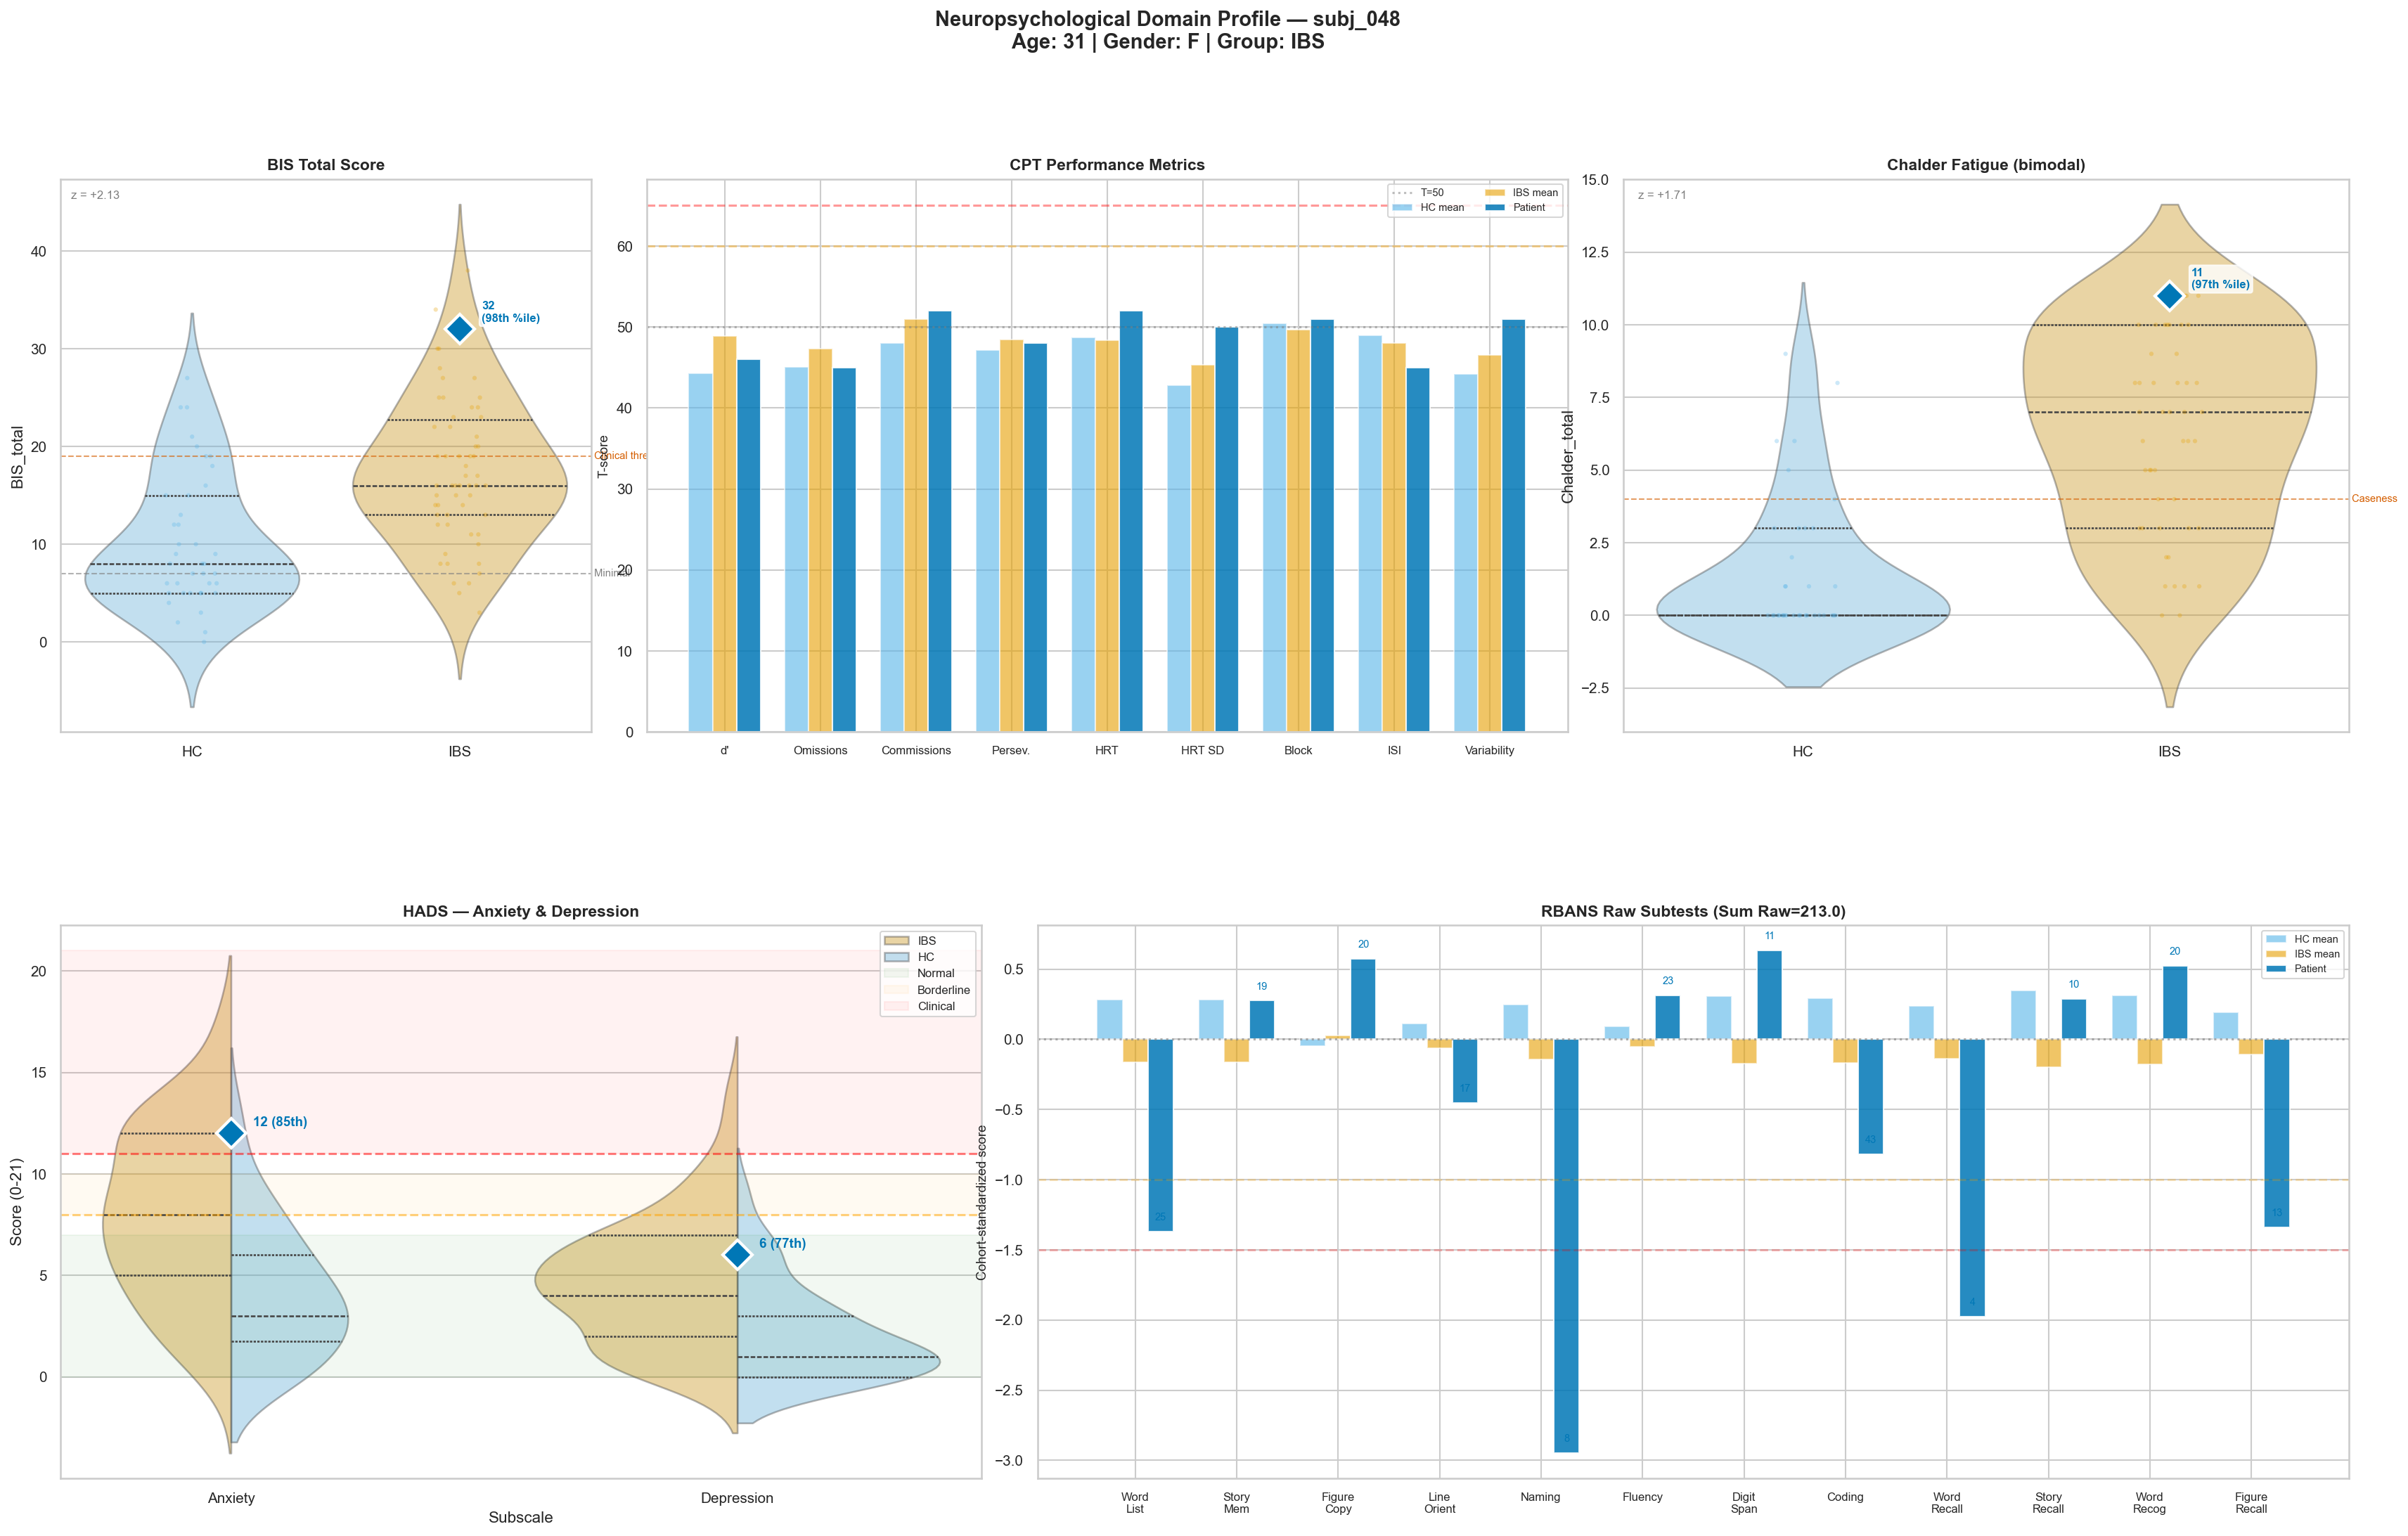
\includegraphics[width=\textwidth]{subj_048_multipanel_clinical.png}
\caption{\textbf{Multi-panel domain profile (clinical detail).}
Each panel shows the cohort distribution (violin plots split by IBS/HC group) with the patient's score marked as a blue diamond.
\textbf{Panel 1 (BIS):} Insomnia total score with clinical threshold (dashed red, $\geq$19) and minimal cutoff (dashed gray).
\textbf{Panel 2 (CPT):} Grouped bars comparing HC mean, IBS mean, and patient T-scores; red/orange triangles flag elevated metrics.
\textbf{Panel 3 (Chalder):} Fatigue bimodal total with caseness threshold (dashed red, $\geq$4).
\textbf{Panel 4 (HADS):} Split violin for Anxiety and Depression; shaded zones mark Normal (green), Borderline (amber), and Clinical (red) ranges.
\textbf{Panel 5 (RBANS):} Raw RBANS subtests displayed on a common cohort-standardized scale, with the patient's raw score annotated above each bar and the broader RBANS Sum Raw shown in the title.
Percentile ranks and z-scores annotate each patient marker. All distributions are within-cohort.}
\end{figure}

\begin{figure}[H]
\centering
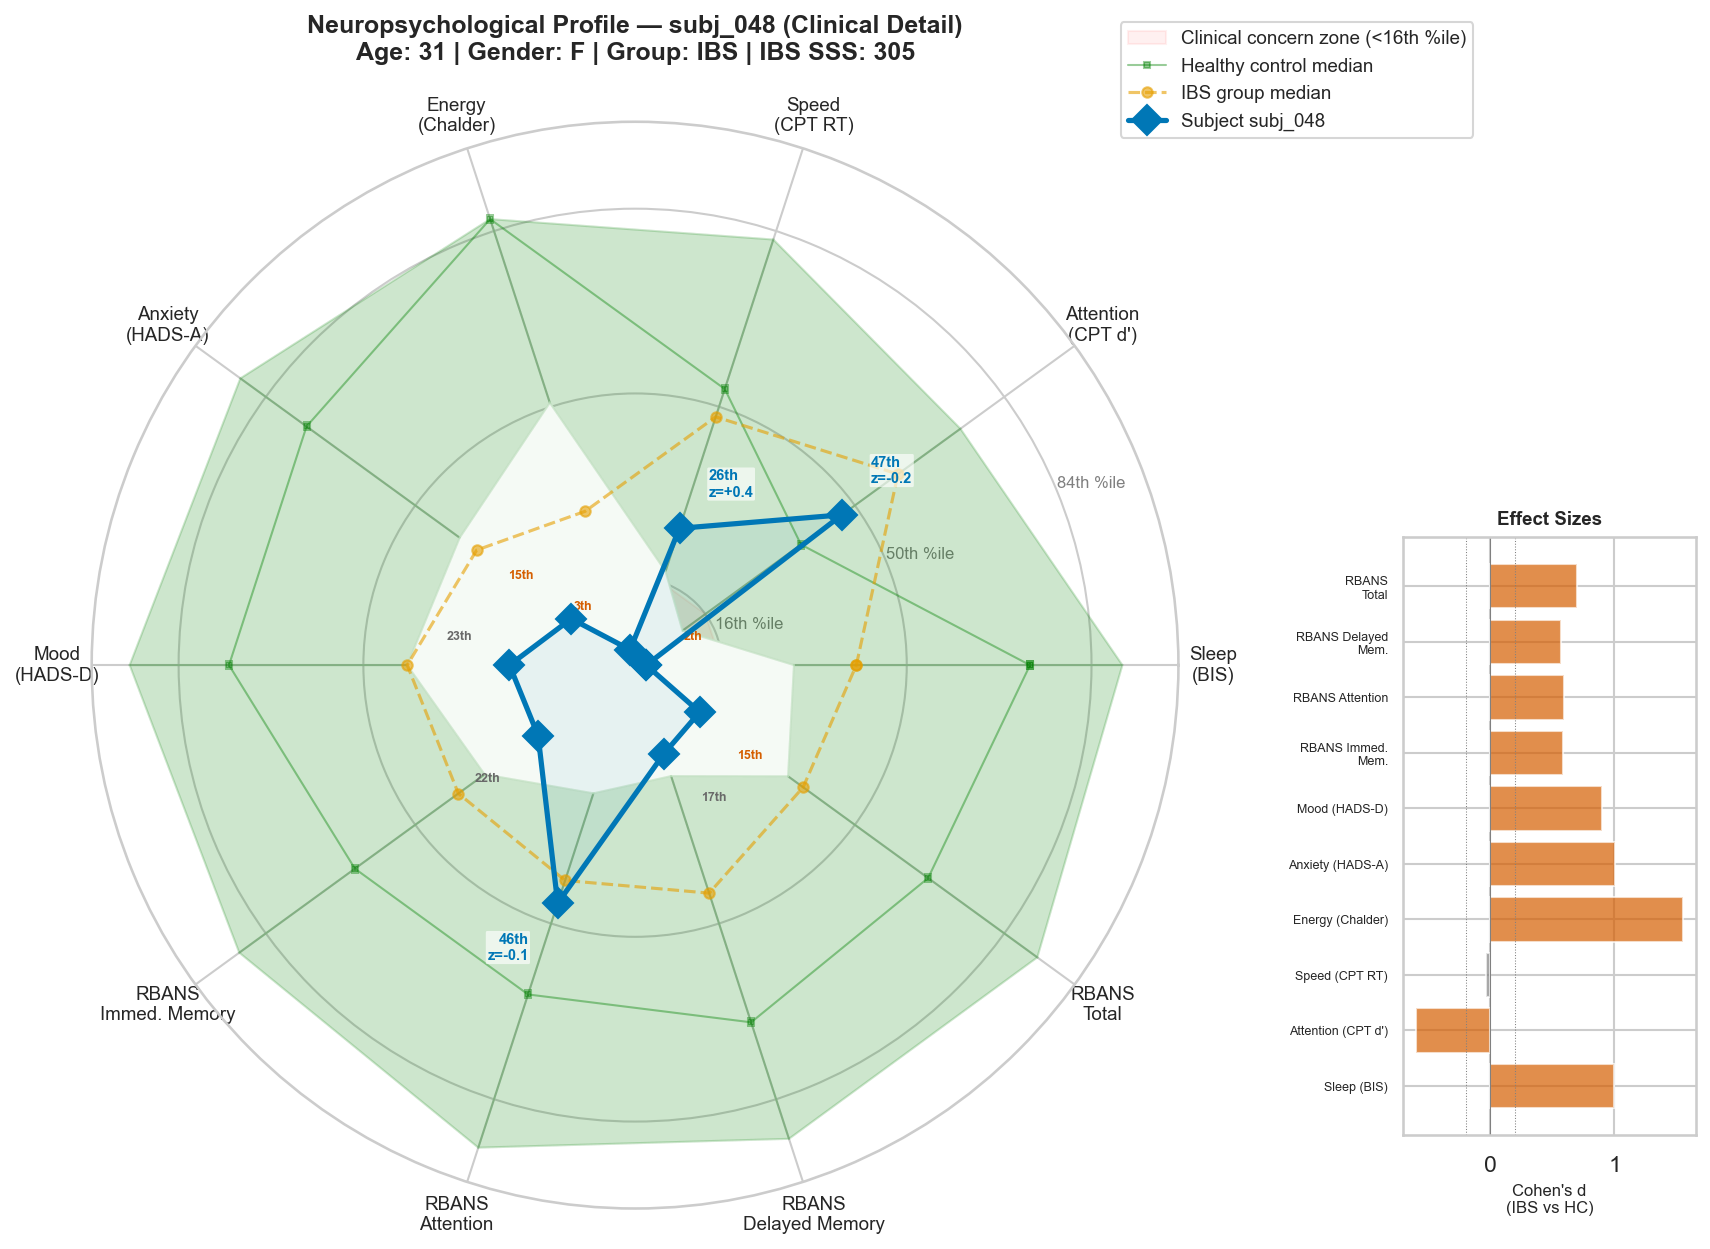
\includegraphics[width=0.85\textwidth]{subj_048_radar_clinical.png}
\caption{\textbf{Radar plot (clinical detail, expanded 10-spoke version).}
Each radial axis represents one domain or subscale, transformed to a common 0--100 percentile-of-wellness scale (higher = better functioning; scales where high raw scores indicate worse outcomes are inverted).
\textbf{Green band:} Healthy control range (16th--84th percentile, i.e.\ $\pm$1~SD).
\textbf{Orange dashed line:} IBS group median profile.
\textbf{Red center zone:} Clinical concern ($<$16th percentile).
\textbf{Blue polygon:} Patient profile, with percentile and z-score annotations at each vertex.
\textbf{Inset (right):} Cohen's $d$ effect sizes for IBS vs.\ HC on each domain. Positive values indicate the IBS group performs worse. $|d| > 0.2$ (small effect) shown in amber; $|d| > 0.5$ (medium effect) in red. This inset contextualizes whether any patient deviations from the healthy range are consistent with the broader IBS group pattern or represent individual-specific findings.}
\end{figure}

% --- B. PHYSICIAN AUDIENCE ---
\subsection{For Referring Physicians}

\begin{figure}[H]
\centering
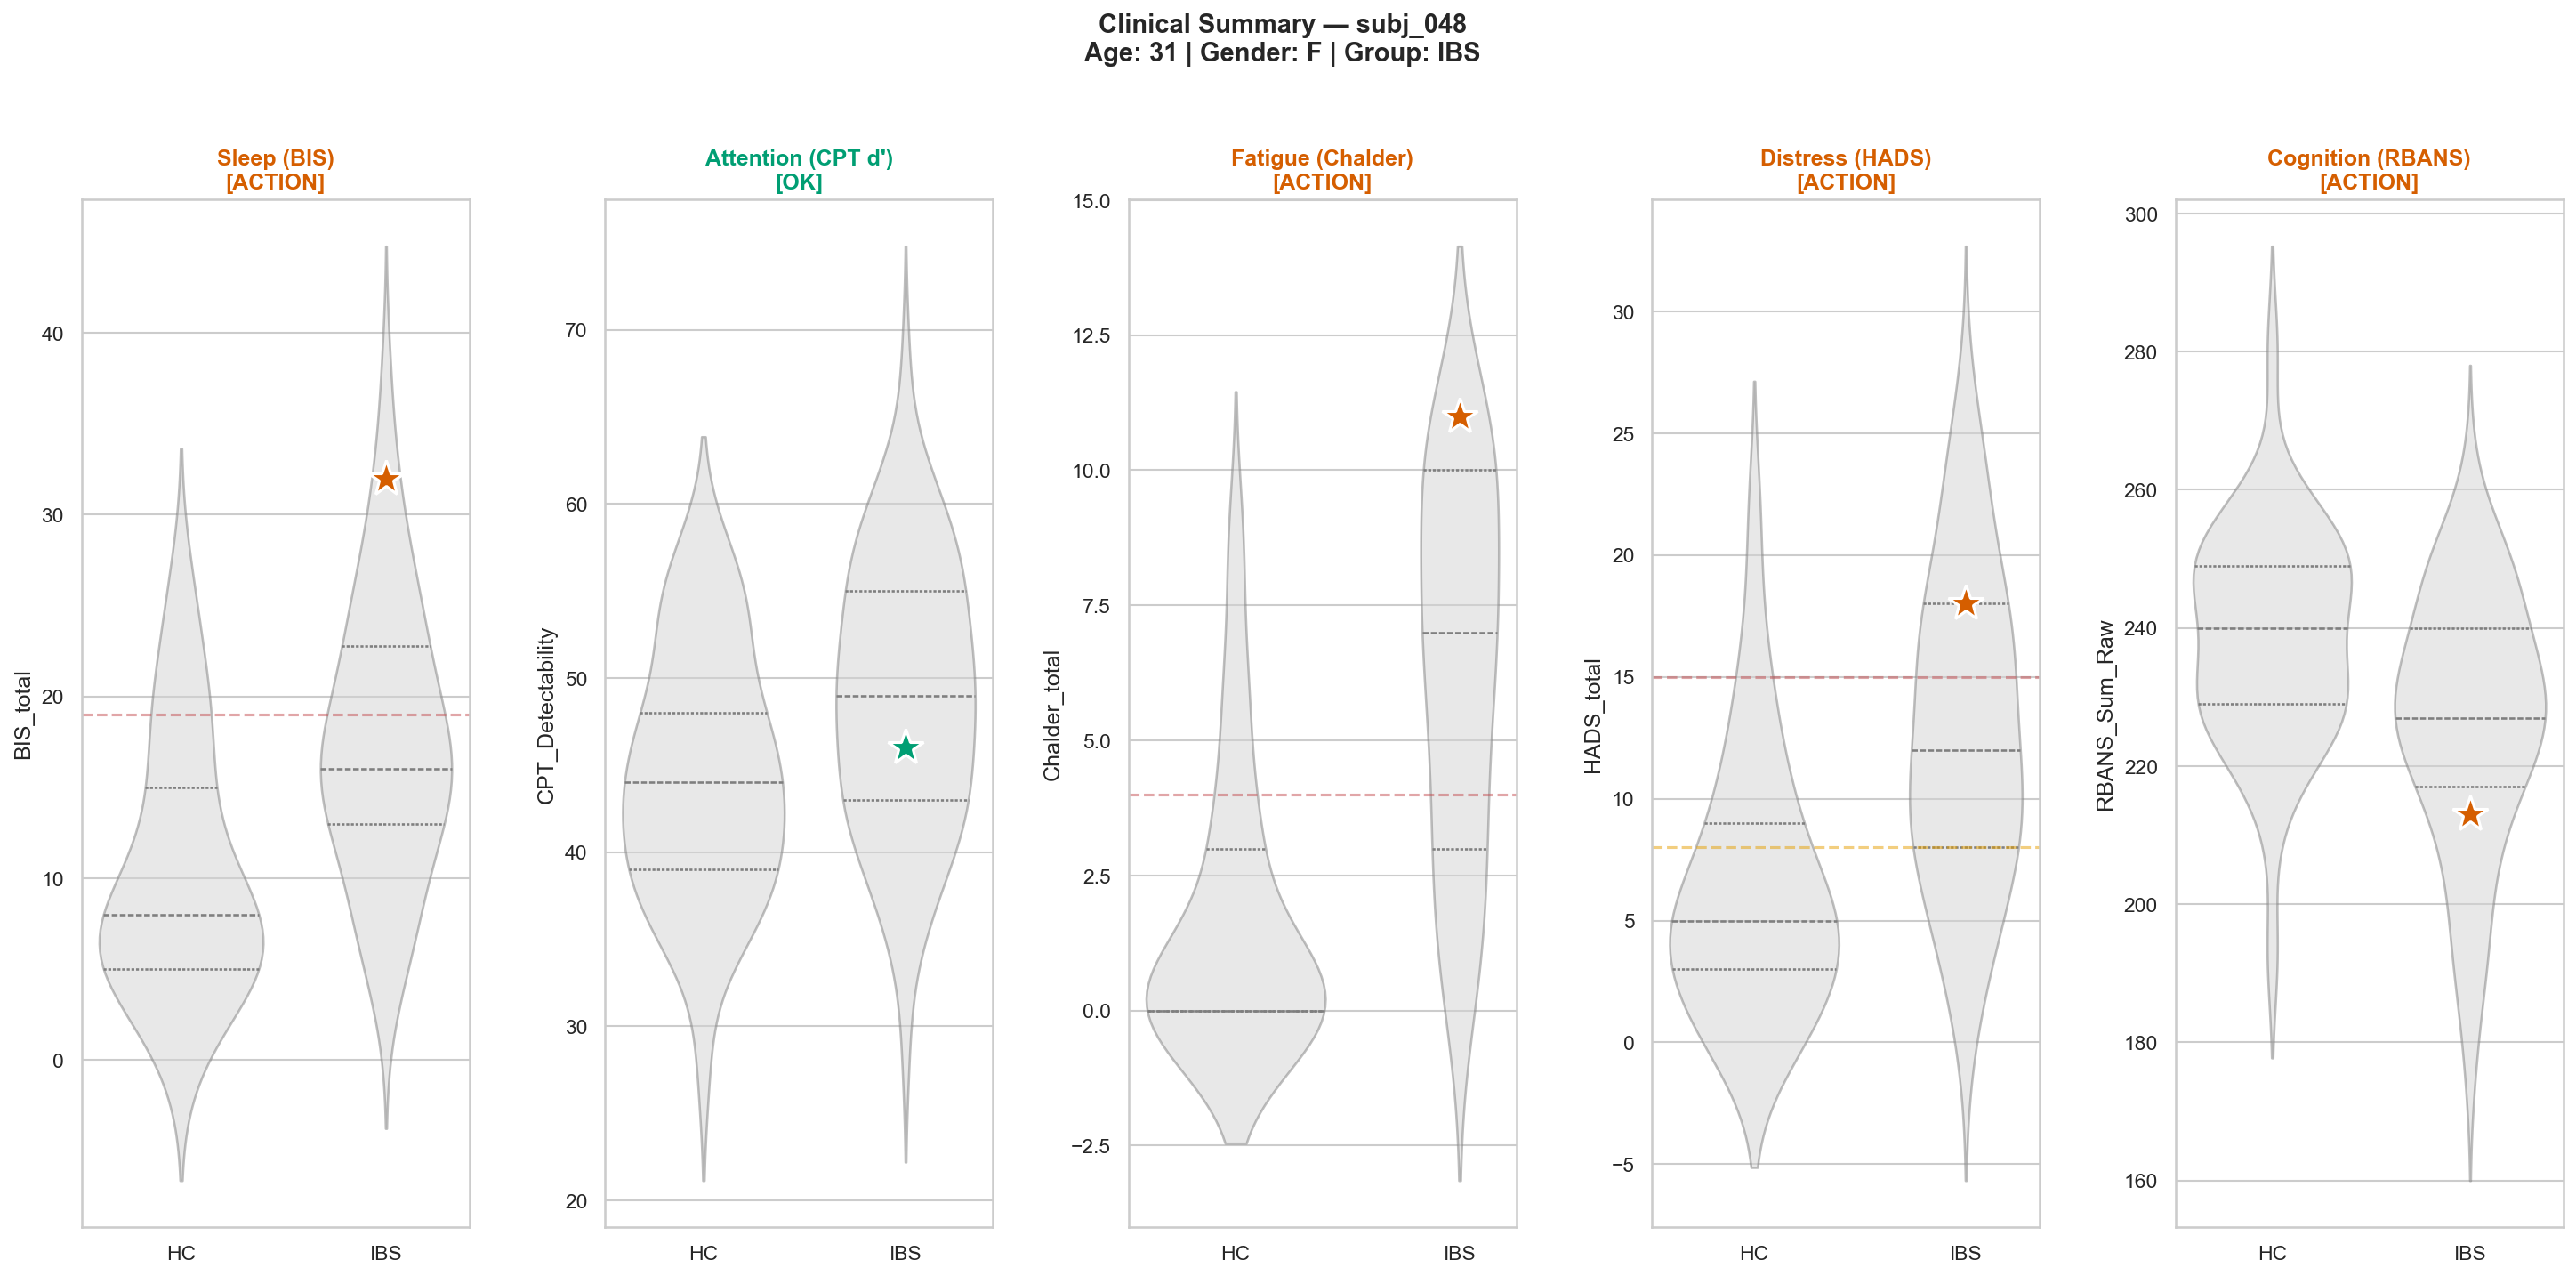
\includegraphics[width=\textwidth]{subj_048_multipanel_physician.png}
\caption{\textbf{Clinical summary (physician view).}
Five-domain overview using simplified violin plots with traffic-light status labels:
\textcolor{clingreen}{\textbf{OK}} ($\geq$50th percentile of wellness),
\textcolor{clinamber}{\textbf{MONITOR}} (16th--49th percentile),
\textcolor{clinred}{\textbf{ACTION}} ($<$16th percentile).
The patient's score is shown as a large star marker. This view is designed for rapid clinical triage: domains marked ACTION warrant immediate intervention or referral; MONITOR domains should be tracked at follow-up.}
\end{figure}

\begin{figure}[H]
\centering
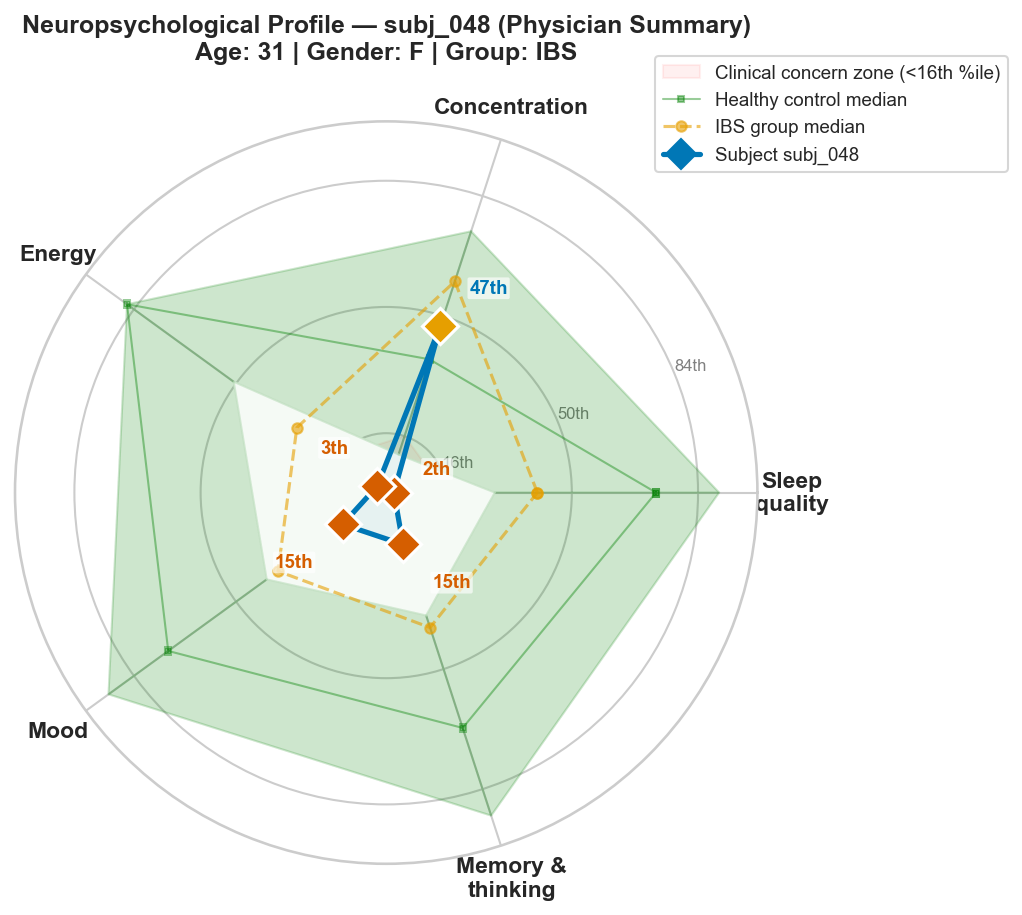
\includegraphics[width=0.75\textwidth]{subj_048_radar_physician.png}
\caption{\textbf{Radar plot (physician view, compact 5-spoke).}
Same percentile-of-wellness normalization as the clinical version, but using five composite domain spokes for rapid pattern recognition.
Vertex colors follow the traffic-light system: green ($\geq$50th), amber (16th--49th), red ($<$16th).
The overall polygon shape reveals whether difficulties are focal (one spoke depressed) or diffuse (multiple spokes depressed).
The green shaded band shows the typical healthy control range for reference.}
\end{figure}

% --- C. PATIENT AUDIENCE ---
\subsection{For the Patient and Close Persons}

\begin{figure}[H]
\centering
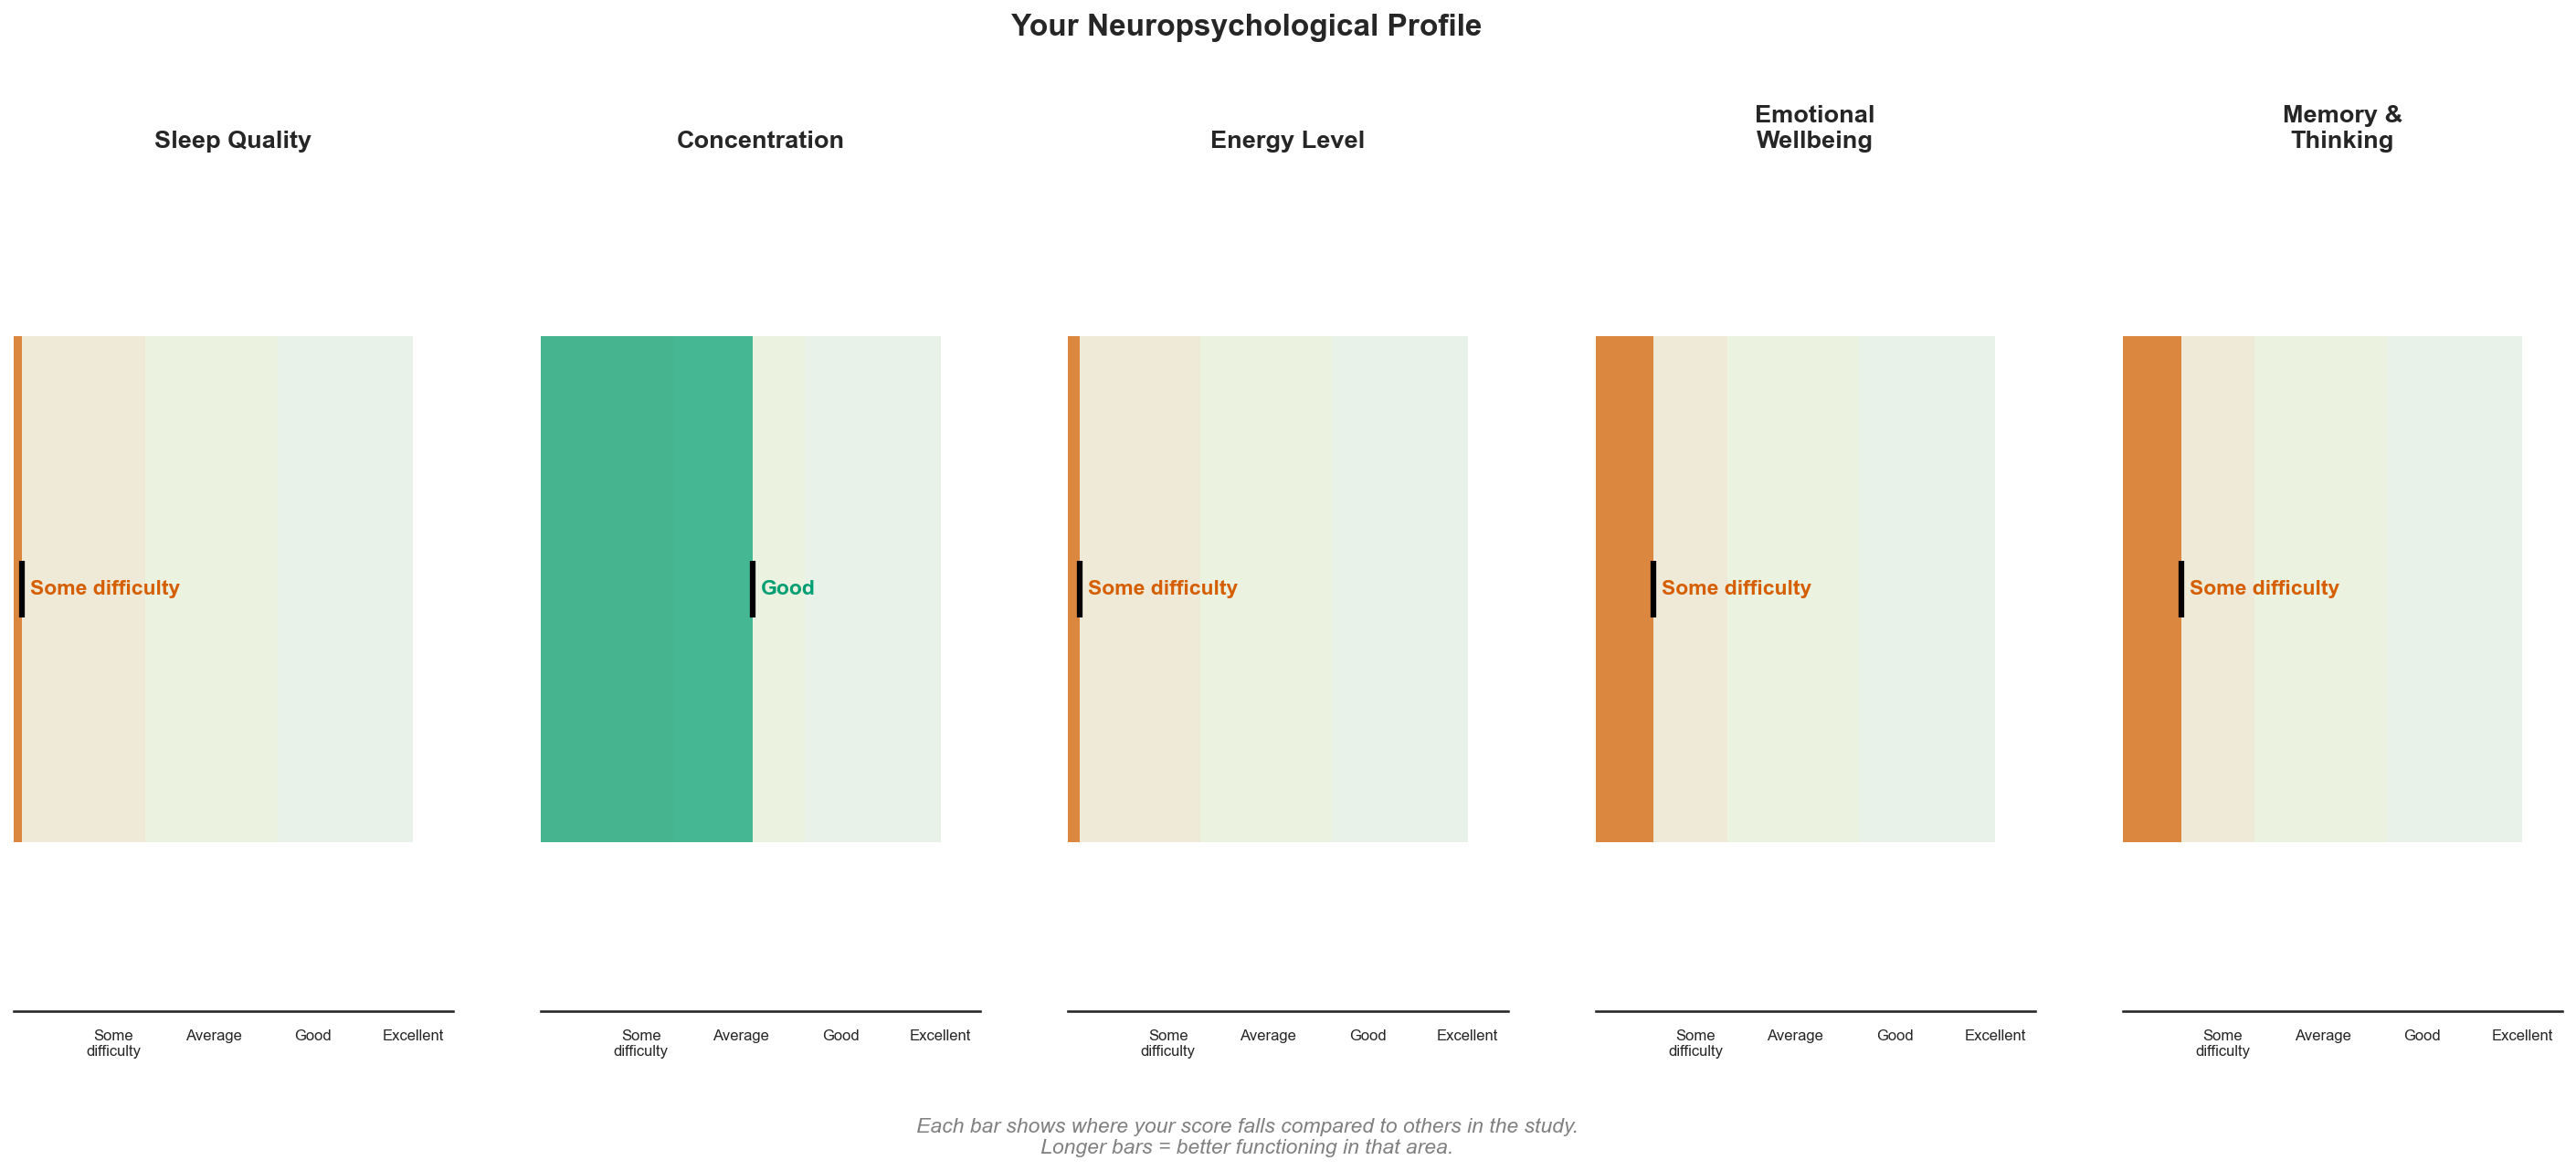
\includegraphics[width=\textwidth]{subj_048_multipanel_patient.png}
\caption{\textbf{Your results at a glance.}
Each horizontal bar shows how your score compares to others in the study. Longer bars (reaching further right) mean better functioning in that area.
The labels ``Some difficulty'', ``Average'', ``Good'', and ``Excellent'' describe where your score falls.
Areas shown in green are going well; areas in amber or red may benefit from support or follow-up.
This chart covers five areas of health: sleep quality, concentration ability, energy levels, emotional wellbeing, and memory and thinking skills.}
\end{figure}

\begin{figure}[H]
\centering
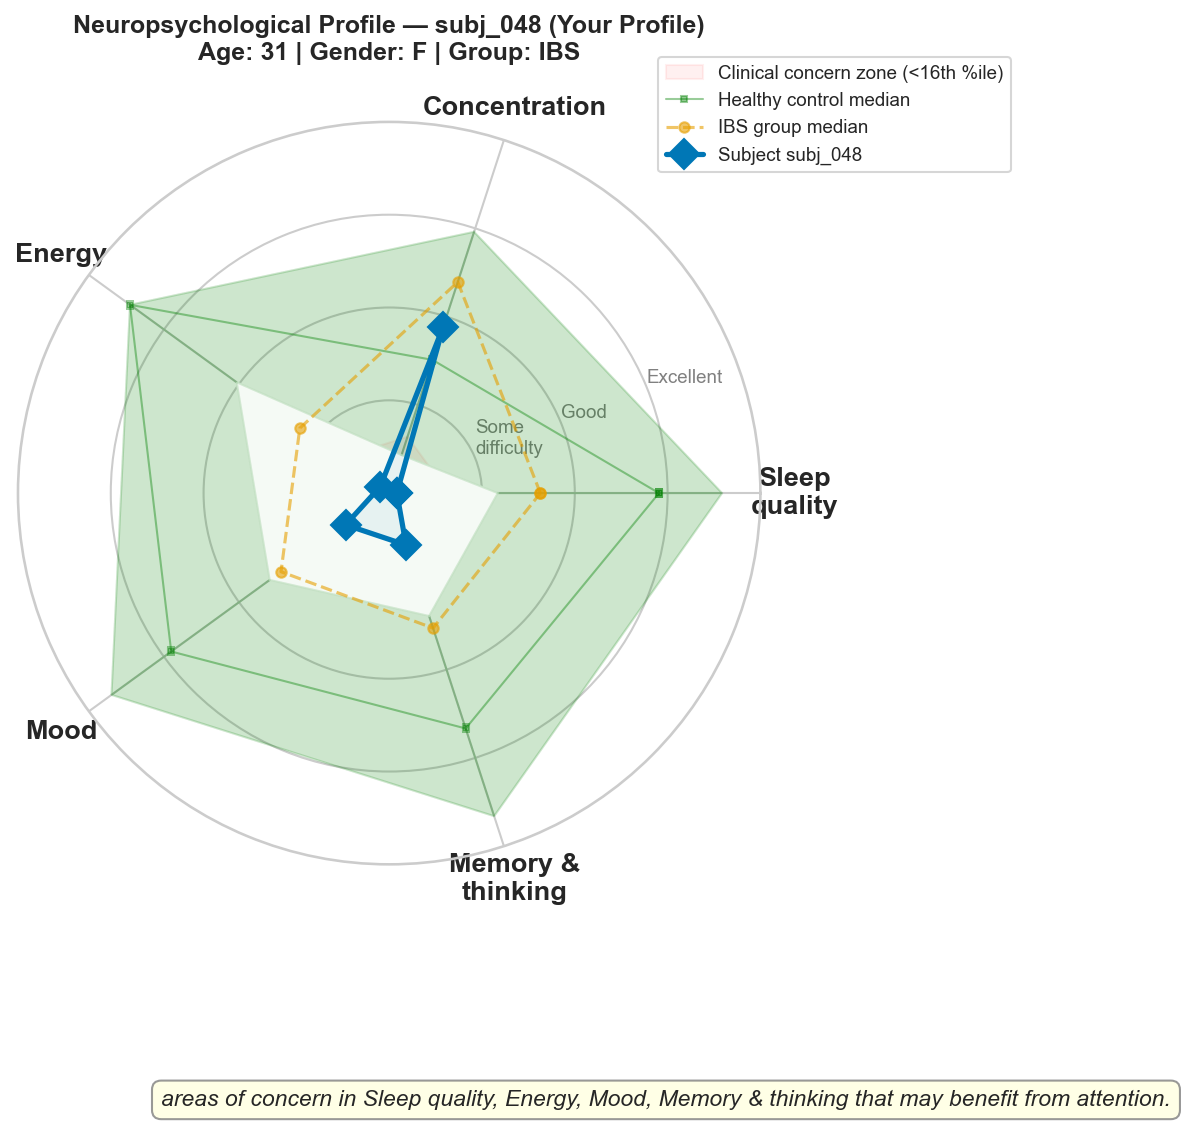
\includegraphics[width=0.75\textwidth]{subj_048_radar_patient.png}
\caption{\textbf{Your overall profile.}
This spider chart shows all five areas together so you can see the overall shape of your strengths and any areas of difficulty.
Points further from the center are better. The green shaded area shows the ``typical healthy range.''
The orange dashed line shows the average for people with IBS.
The blue shape is your personal profile.
The sentence at the bottom provides a plain-language summary of what the chart shows.}
\end{figure}

% ================================================================
\vfill
\noindent\rule{\textwidth}{0.4pt}\\
\small\textit{This report was generated by an AI-based neuropsychological analysis pipeline.
All interpretations should be reviewed and validated by a qualified clinical neuropsychologist.
Findings are based on cross-sectional cohort data (N=105). CPT values remain norm-referenced T-scores, whereas the RBANS section in this standalone March 16 pipeline uses raw subtests and cohort-standardized summaries rather than external age-corrected RBANS index norms.
Clinical cutoffs follow established guidelines: HADS (Zigmond \& Snaith, 1983; Bjelland et al., 2002),
BIS (Pallesen et al., 2008), Chalder Fatigue Scale (Chalder et al., 1993),
RBANS (Randolph, 1998), CPT-3 (Conners, 2014).}

\end{document}
